\chapter{Analysis}
After utilizing the AUSAlib tools, the data is ready to be analyzed. Even though the theory dictates that a decay will consist of two \al-particles and one \be-particles, it is not realistic to just assume that each detected event will consist only of this configuration of particles. \\
Therefore we need some cut on what events we will allow through to the analysis. Specifically we are going to impose 3 cuts on the data, a angular cut, a momentum cut and a multiplicity cut.


\section{Angular cut}
When a particle hits a given detector, we have no real knowledge of what particle it is. 
Therefore we need to use other properties of the decay to determine the particle type. 
When \isotope[8][]Be decays, and produces the two \al-particles, it will do so under conservation of momentum. The decay in any direction, but the angle between $\theta$ them will be close to  $180\degree$, or $\cos(\theta) \geq -1$. Therefore the first cut that we give to the data, is that two of the particles that are \al candidates, must have a mutual angle of close to $180\degree$.\\


On \cref{fig:cosAll} a plot of all the the mutual angles are shown. A quick glance will give that most particles will have mutual angle of close to $180\degree$. 

\begin{figure}[h]
	\centering
	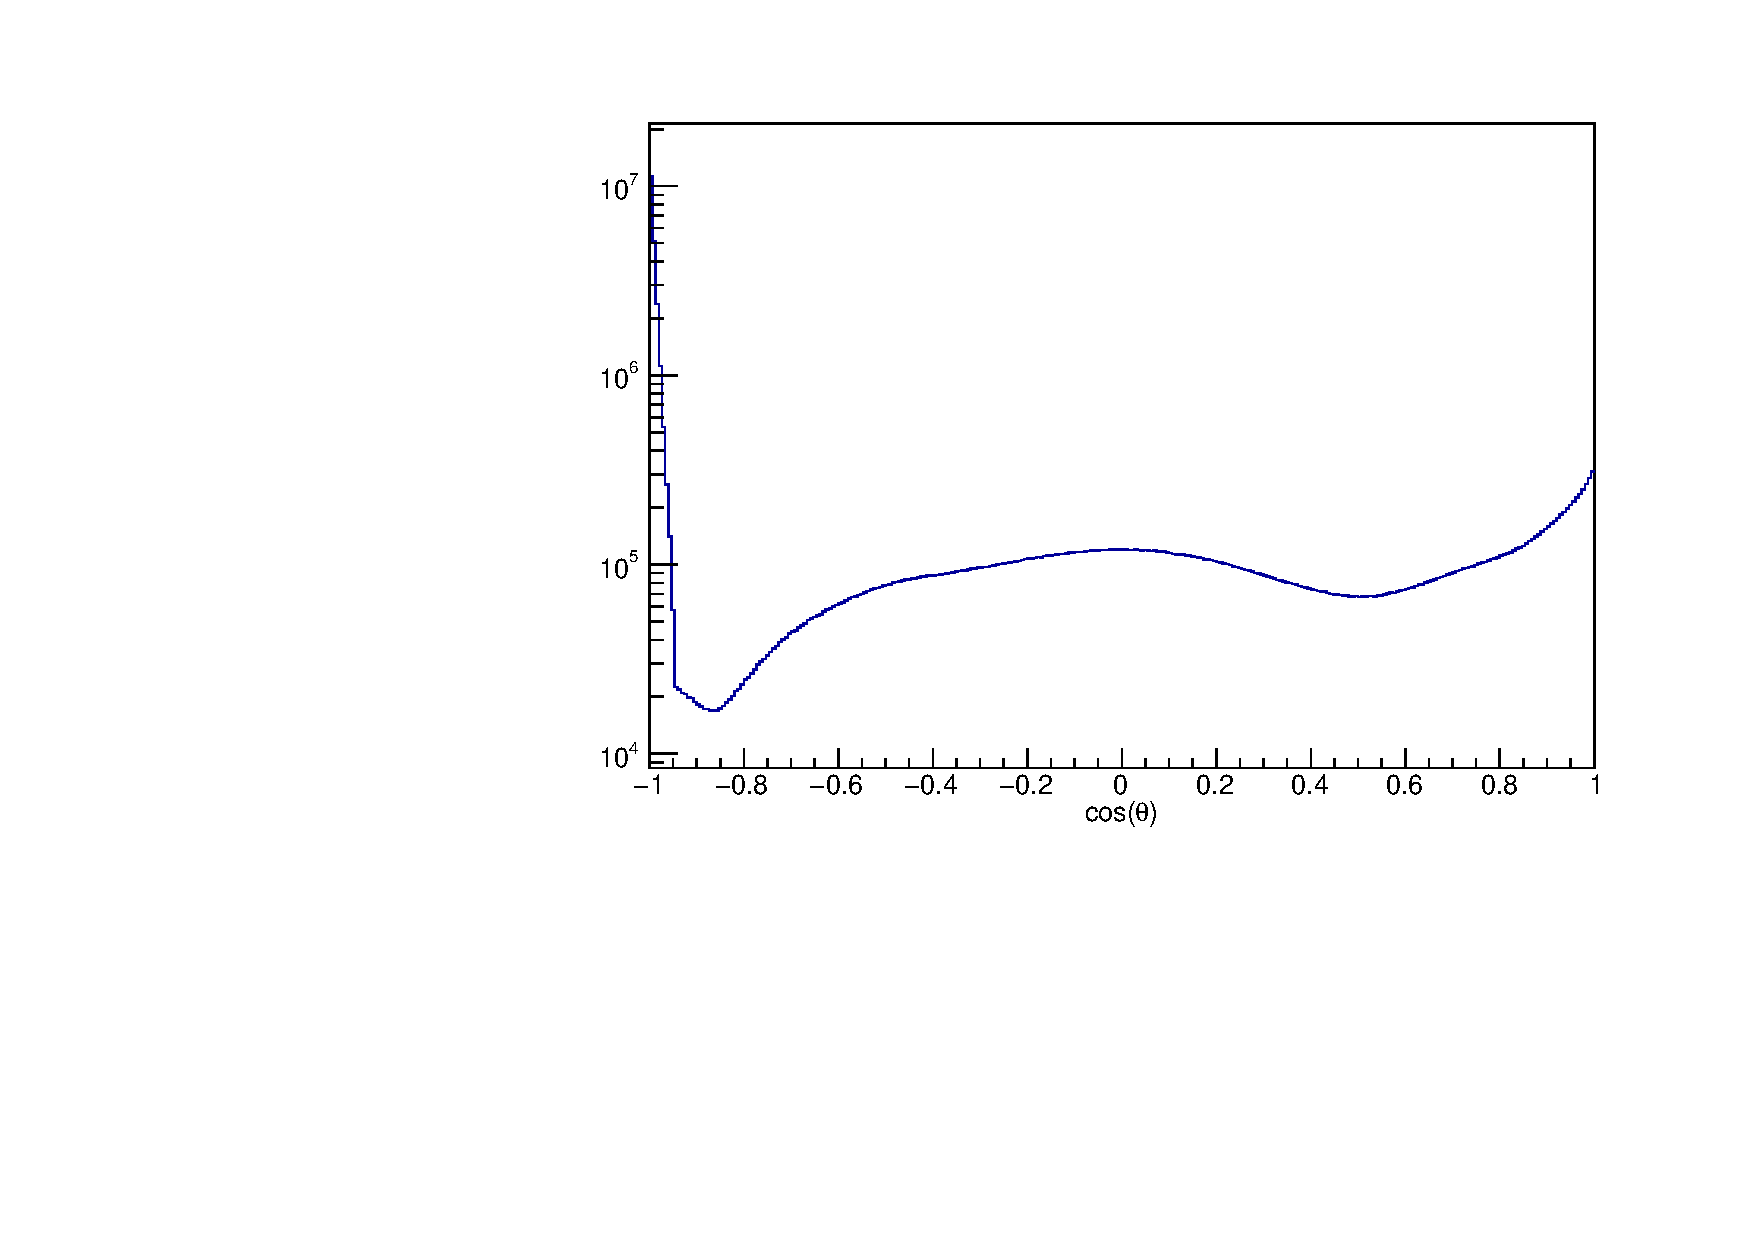
\includegraphics[width=\linewidth]{../figures/cosang.pdf}
	\caption{A plot of all the mutual angles between the \al-particle candidates.}
	\label{fig:cosAll}
\end{figure}

By looking at this, we see that most of the angles will lie close to $180\degree$, and now we must decide excatly where to do the cutoff. 
By taking a sharp cutoff at $\cos(\theta) \geq -0.99$, we will exclude a great deal of good measurements.




\section{Momentum cut}

\section{Multiplicity cut}